
\section{PAML Data Model}\label{sec:model}

The section describes the PAML data model in detail.  
OPIL classes are in general organized in pairs, one for specifying the interface to a protocol, the other for making requests to execute protocol via that interface.
As such, this section is also organized in pairs, first each interface class, then the complementary request class.

\subsection{Protocol}
\label{sec:Protocol}

The \paml{Protocol} class represents an executable protocol.


\begin{center}
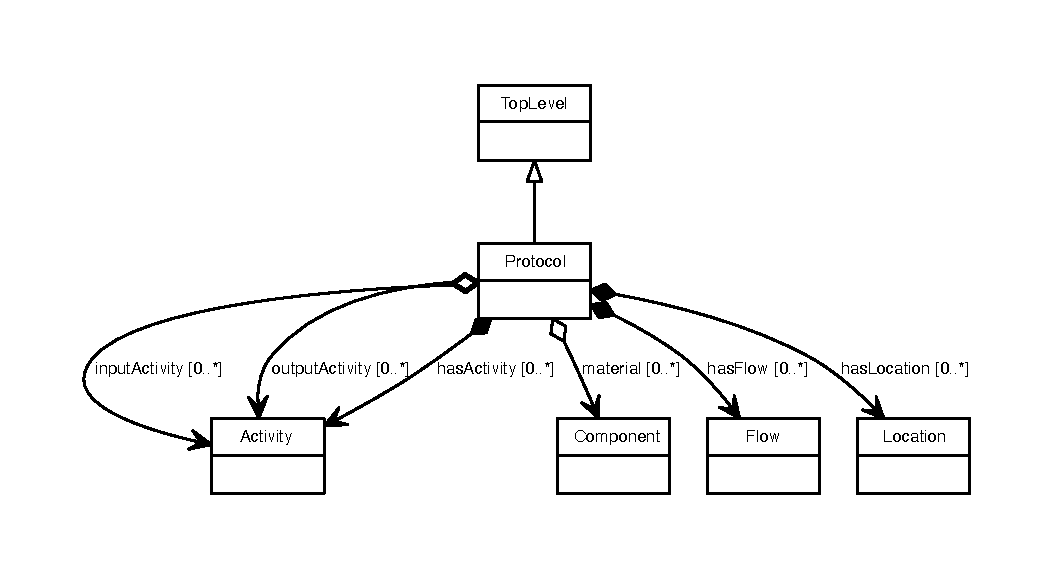
\includegraphics[scale=0.8]{uml/Protocol_abstraction_hierarchy.pdf}
%\caption[]{Diagram of the \opil{ProtocolInterface} class and its associated properties}
%\label{uml:ProtocolInterface}
\end{center}


\subsection{Activity}
\label{sec:Activity}

%\begin{figure}[ht]
%\begin{center}
%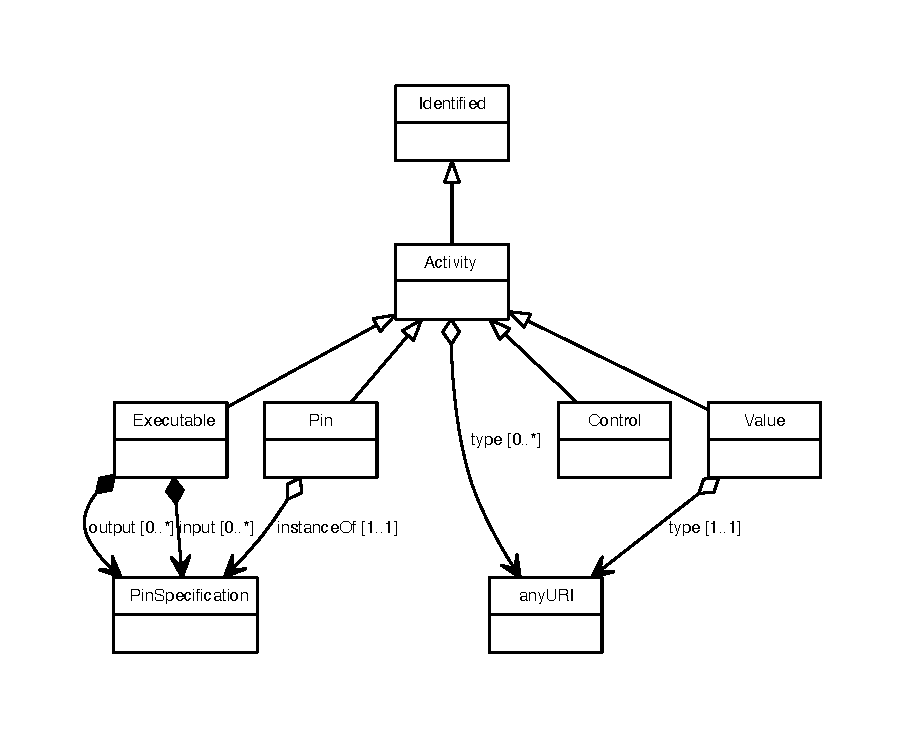
\includegraphics[scale=0.8]{uml/Activity_abstraction_hierarchy.pdf}
%%\caption[]{Diagram of the \opil{ProtocolInterface} class and its associated properties}
%%\label{uml:ProtocolInterface}
%\end{center}
%


\begin{center}
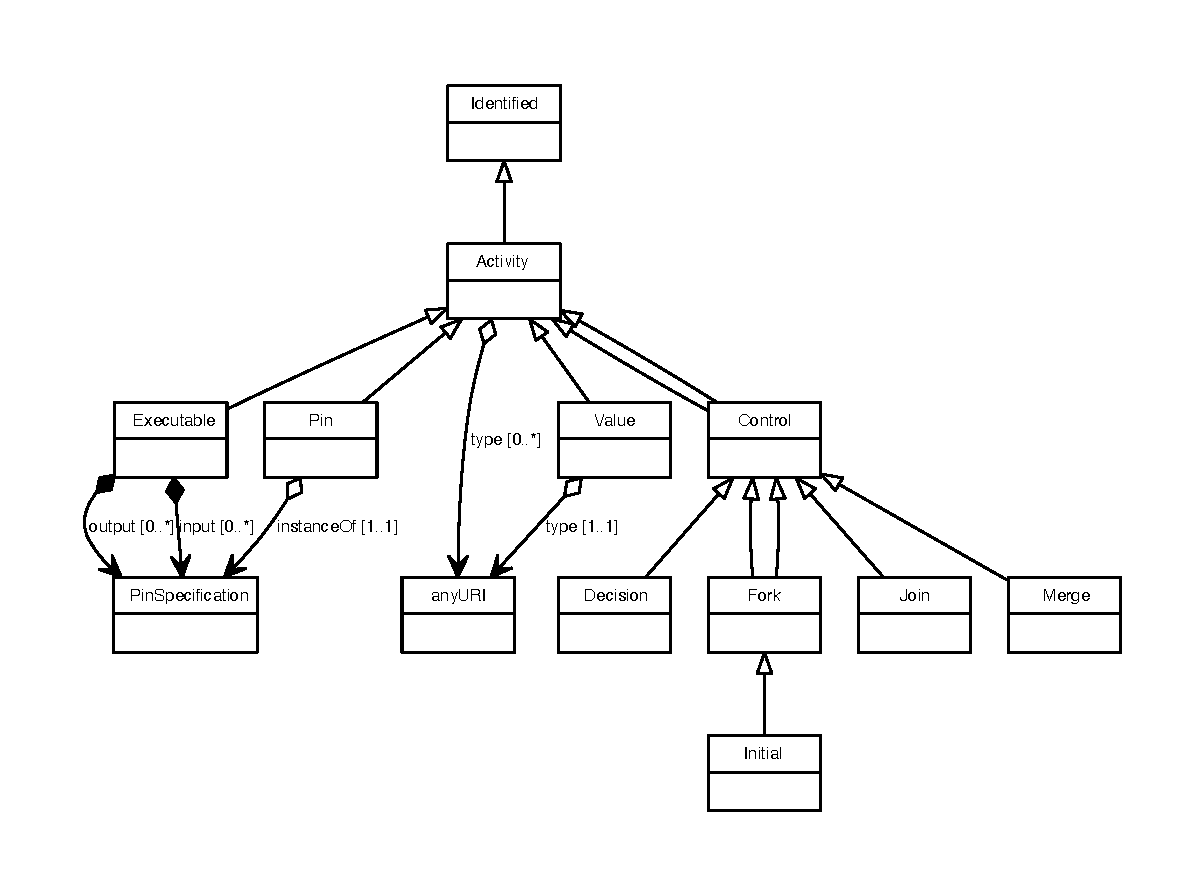
\includegraphics[scale=0.8]{uml/Initial_abstraction_hierarchy.pdf}
%\caption[]{Diagram of the \opil{ProtocolInterface} class and its associated properties}
%\label{uml:ProtocolInterface}
\end{center}



\begin{center}
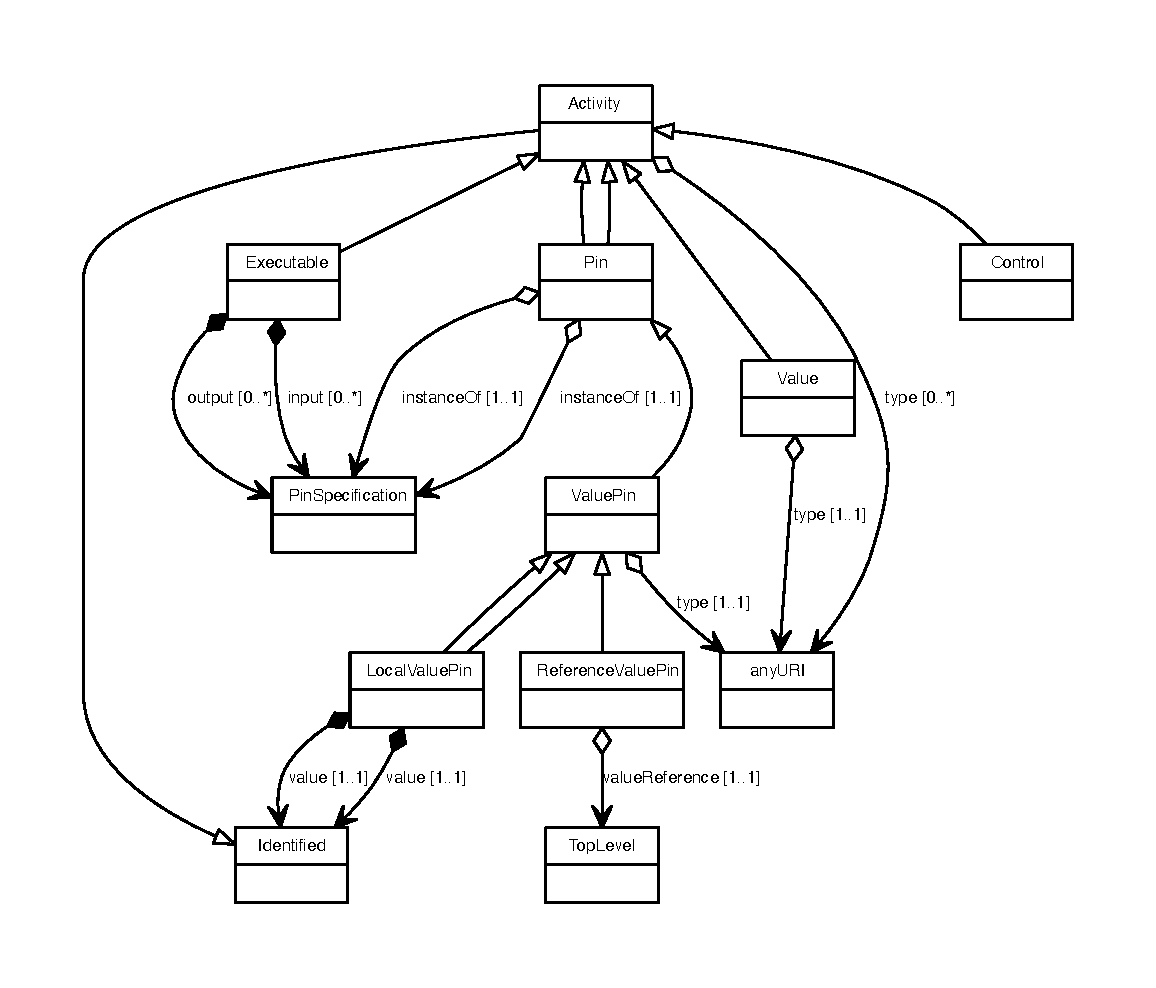
\includegraphics[scale=0.8]{uml/LocalValuePin_abstraction_hierarchy.pdf}
%\caption[]{Diagram of the \opil{ProtocolInterface} class and its associated properties}
%\label{uml:ProtocolInterface}
\end{center}



\begin{center}
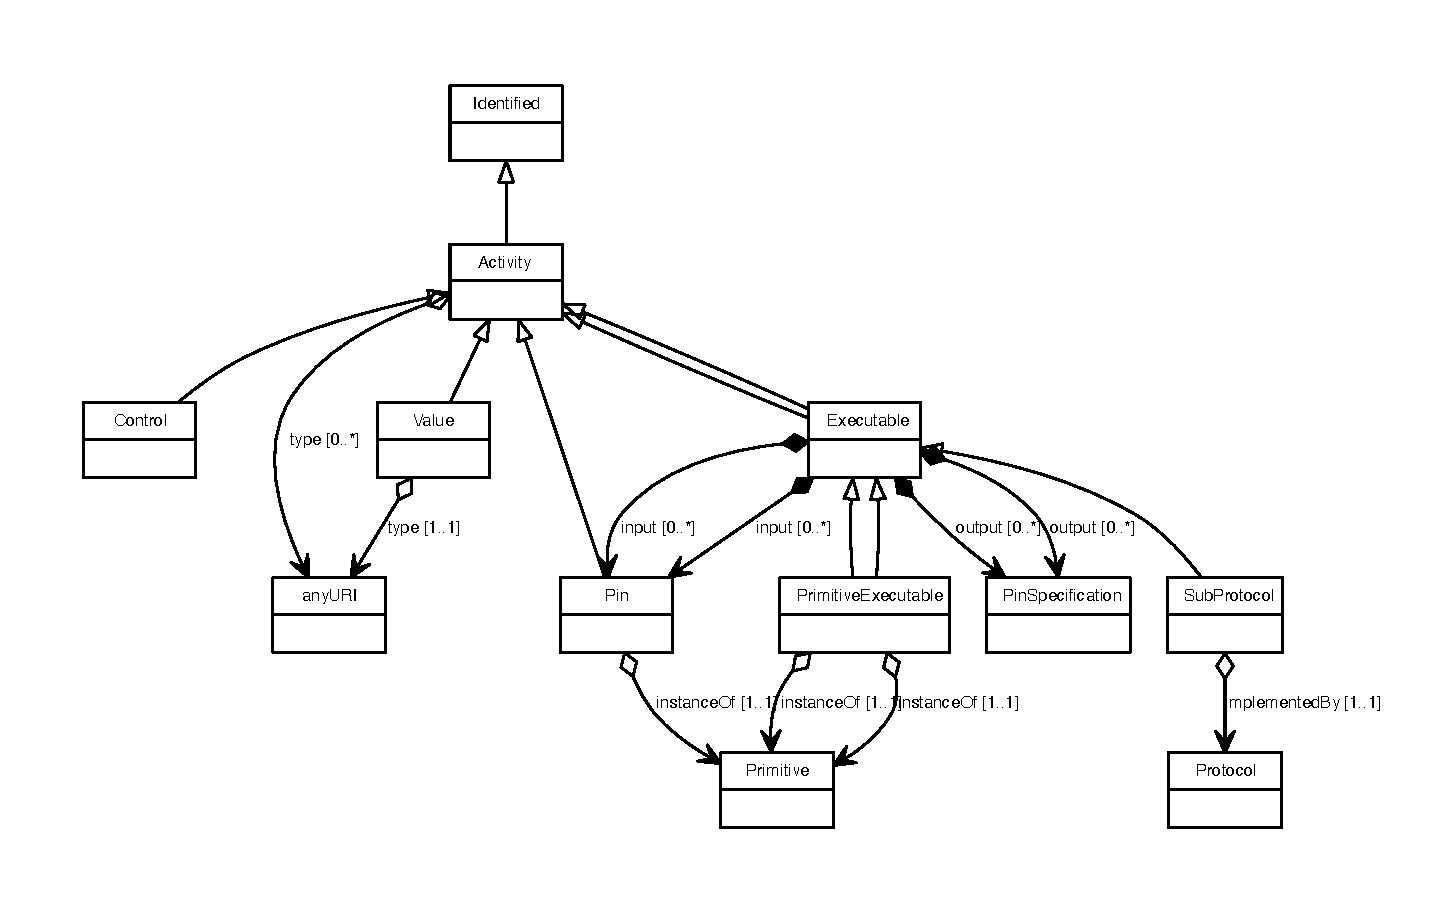
\includegraphics[width=\textwidth]{uml/PrimitiveExecutable_abstraction_hierarchy.pdf}
%\caption[]{Diagram of the \opil{ProtocolInterface} class and its associated properties}
%\label{uml:ProtocolInterface}
\end{center}



\begin{center}
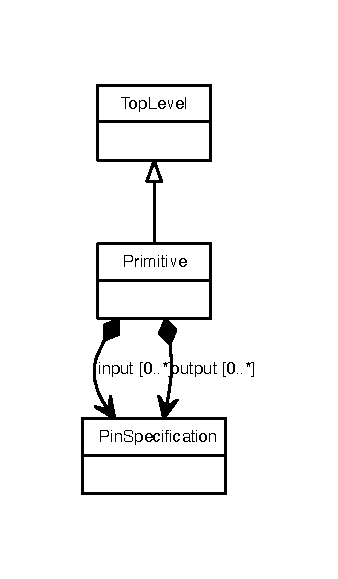
\includegraphics[scale=0.8]{uml/Primitive_abstraction_hierarchy.pdf}
%\caption[]{Diagram of the \opil{ProtocolInterface} class and its associated properties}
%\label{uml:ProtocolInterface}
\end{center}



\begin{center}
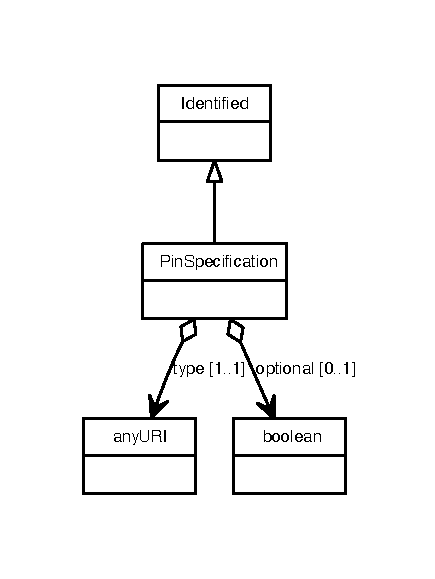
\includegraphics[scale=0.8]{uml/PinSpecification_abstraction_hierarchy.pdf}
%\caption[]{Diagram of the \opil{ProtocolInterface} class and its associated properties}
%\label{uml:ProtocolInterface}
\end{center}


\subsection{Flow}
\label{sec:Flow}



\begin{center}
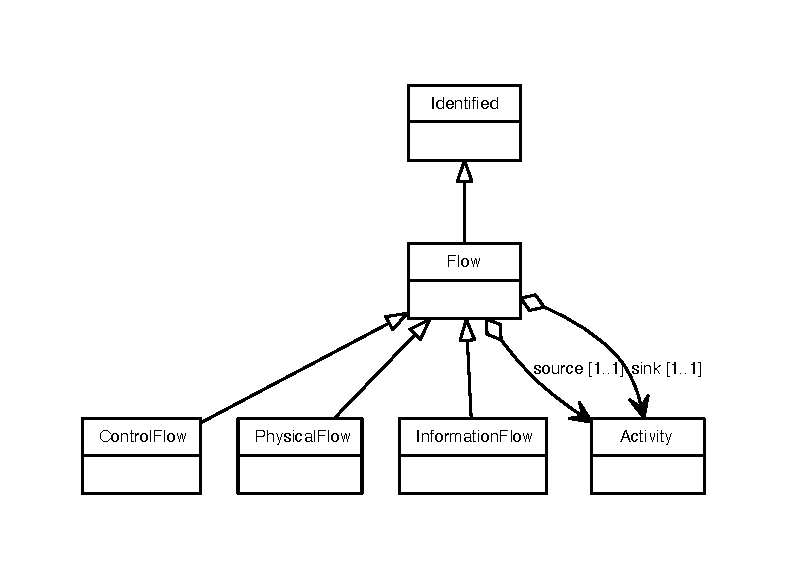
\includegraphics[scale=0.8]{uml/Flow_abstraction_hierarchy.pdf}
%\caption[]{Diagram of the \opil{ProtocolInterface} class and its associated properties}
%\label{uml:ProtocolInterface}
\end{center}


\subsection{Location}
\label{sec:Location}


\begin{center}
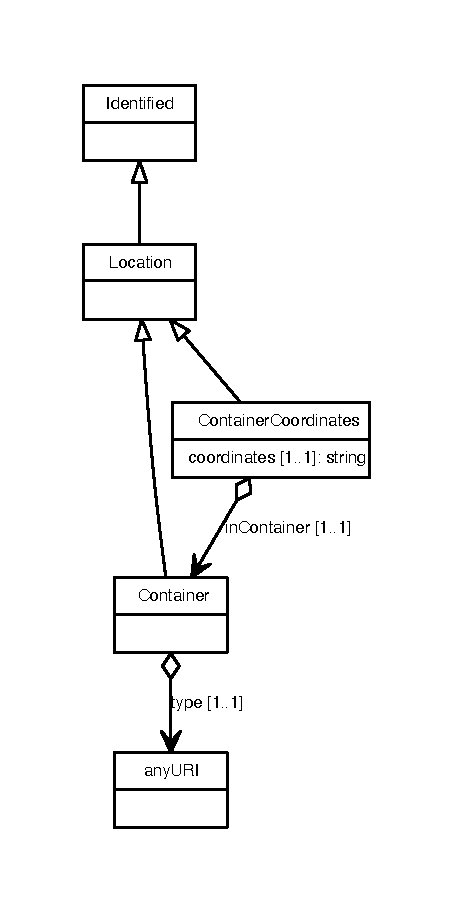
\includegraphics[scale=0.8]{uml/Location_abstraction_hierarchy.pdf}
%\caption[]{Diagram of the \opil{ProtocolInterface} class and its associated properties}
%\label{uml:ProtocolInterface}
\end{center}


\subsection{LocatedSamples}
\label{sec:LocatedSamples}


\begin{center}
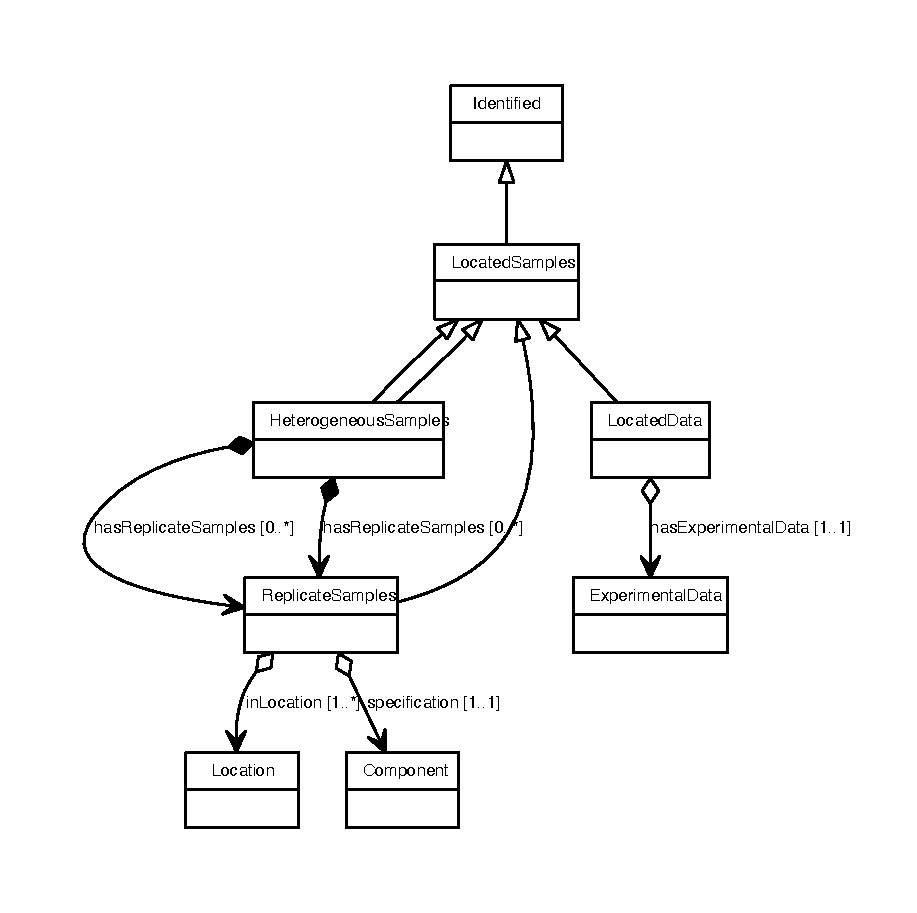
\includegraphics[scale=0.8]{uml/HeterogeneousSamples_abstraction_hierarchy.pdf}
%\caption[]{Diagram of the \opil{ProtocolInterface} class and its associated properties}
%\label{uml:ProtocolInterface}
\end{center}



%%% Local Variables:
%%% mode: latex
%%% TeX-master: "paml"
%%% End:
